\documentclass[a4paper, 12pt]{report}
\usepackage{graphicx}
\usepackage[french]{babel}
\usepackage{caption}
\usepackage[utf8]{inputenc}
\usepackage[T1]{fontenc}
\usepackage{multirow}
\usepackage{listings}
\usepackage{float}
\usepackage{url}
\usepackage[french]{algorithm}
\usepackage{style/myalgorithm}
\usepackage{amsmath,amsfonts,amssymb}
\newcommand{\fBm}{\emph{fBm}~}
\newcommand{\etal}{\emph{et al.}~}
\newcommand{\glAd}{\emph{GL4D}~}
\newcommand{\apiopengl}{API OpenGL\textsuperscript{\textregistered}~}
\newcommand{\opengl}{OpenGL\textsuperscript{\textregistered}~}
\newcommand{\opengles}{OpenGL\textsuperscript{\textregistered}ES~}
\newcommand{\clang}{langage \texttt{C}}
\newcommand{\codesource}{\textsc{Code source}~}
\floatstyle{ruled}
\newfloat{programslist}{htbp}{locs}
\newcommand{\listofprograms}{\listof{programslist}{Liste des codes source}}
\newcounter{program}[subsection]
\renewcommand{\theprogram}{\arabic{chapter}.\arabic{program}}

\newenvironment{program}[1]{
  \if\relax\detokenize{#1}\relax
  \gdef\mycaption{\relax}
  \else
  \gdef\mycaption{#1}
  \fi
  \refstepcounter{program}
  \addcontentsline{locs}{section}{#1}
  \footnotesize
}{
  \begin{description}
    \item[\codesource \theprogram]--~\mycaption
  \end{description}
}

\begin{document}
\begin{titlepage}
  \begin{center}
    \begin{tabular*}{\textwidth}{l@{\extracolsep{\fill}}r}
      
\includegraphics[height=1.5cm]{images/m2ise.png}
    \end{tabular*}
    \small 
    \rule{\textwidth}{.5pt}~\\
    \large 
    \textsc{Université Paris 8 - Vincennes à Saint-Denis}\vspace{0.5cm}\\
    \textbf{Master Informatique des Systèmes Embarqués}\vspace{3.0cm}\\
    \Large
    \textbf{Memoire de projet tuteuré}\vspace{1.5cm}\\
    \large
    \textbf{Fakhri \textsc{YAHIAOUI} - Roman \textsc{BOURSIER}}\vspace{1.5cm}\\
    Date de soutenance : le 09/06/2020\vspace{1.75cm}\\
  \end{center}\vspace{1.5cm}~\\
  \begin{tabular}{ll}
    \hspace{-0.45cm}Tuteur -- Université~:~&~Farès \textsc{BELHADJ}\\
  \end{tabular}
\end{titlepage}
\chapter*{Résumé}
\markboth{\sc Résumé}{}
\addcontentsline{toc}{chapter}{Résumé} 

A faire en dernier ...


\chapter*{Remerciements}
\markboth{\sc Remerciements}{}
\addcontentsline{toc}{chapter}{Remerciements} 

Idem ...

%% Table des matières
\tableofcontents

\chapter*{Introduction}
\markboth{\sc Introduction}{}
\addcontentsline{toc}{chapter}{Introduction}


Dans le cadre de notre projet de fin d'étude, nous souhaitons utiliser un modèle de Deep Learning, afin de produire un moteur de rendu capable d’adopter une stylisation « type » telle que la peinture chinoise. Dans un premier temps, il s’agira de proposer un modèle d’abstraction des peintures sélectionnées comme base d’apprentissage et d’utiliser le couple « peinture originale » / « abstraction » pour l’entraînement. Par la suite, un moteur de rendu d’abstractions sera connecté au réseau profond qui produira une peinture sur la base de l’abstraction.

Le modèle généré devra d'une part adopter la stylisation retenue mais aussi interpréter l'abstraction d'origine.

\section{Problématique}

La "traduction image-image" (Image-to-image translation) permet d'apprendre le mapping entre une image d'entrée et de sortie. En Figure \ref{fig-pix2pix}, nous testons la génération d'un paysage à partir d'un croquis simple. En Figure \ref{fig-pix2pix-fail}, c'est un échec.

\begin{center}
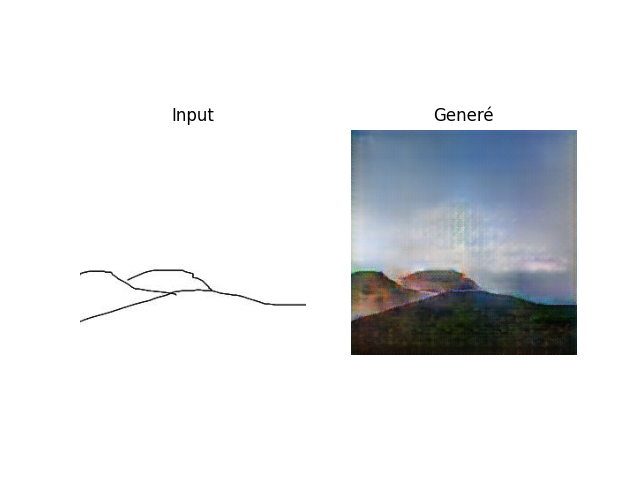
\includegraphics[width=0.7\linewidth]{images/pix2pix-t1.png}
\captionof{figure}{Test du framework pix2pix \cite{DBLP:journals/corr/IsolaZZE16} sur notre dataset composé de photos de paysages, labellisées en appliquant un filtre Canny \cite{4767851} sur chacune d'elles.}
\label{fig-pix2pix}
\end{center}

\begin{center}
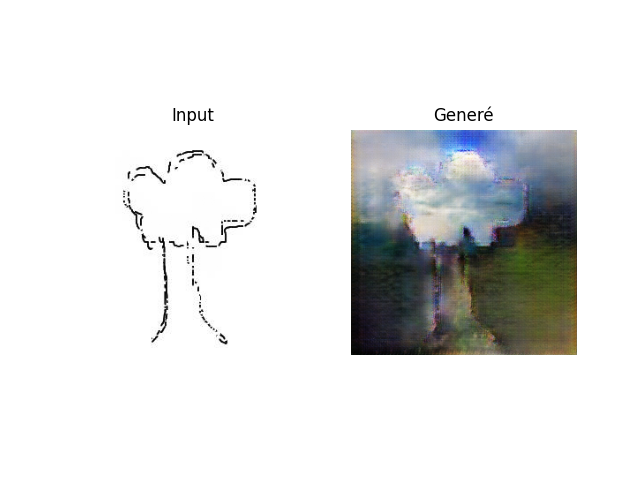
\includegraphics[width=0.7\linewidth]{images/pix2pix-fail.png}
\captionof{figure}{Utilisation du même modèle avec une abstraction d'arbre}
\label{fig-pix2pix-fail}
\end{center}

Comme évoqué dans \cite{DBLP:journals/corr/abs-1805-00247} les algorithmes du type "traduction image-image" se basent essentiellement sur la corrélation d'une image à l'autre, et relève d'un apprentissage supervisé. Le rendu en Figure \ref{fig-pix2pix-fail} s'explique par la nature du dataset et par la distance importante qui sépare une abstraction d'une photo. 

En Figure \ref{fig-croquis} nous avons demandé à plusieurs personnes de dessiner schématiquement un paysage composé de montagnes et d'arbres, éléments courant de la peinture chinoise. Ces dessins sont des abstractions, que nous souhaitons traduire en peintures chinoises.

\begin{center}
  \centering
  \begin{tabular}{ccc}
    \includegraphics[angle=90, height=0.15\textheight]{images/croquis_1.jpg}&
    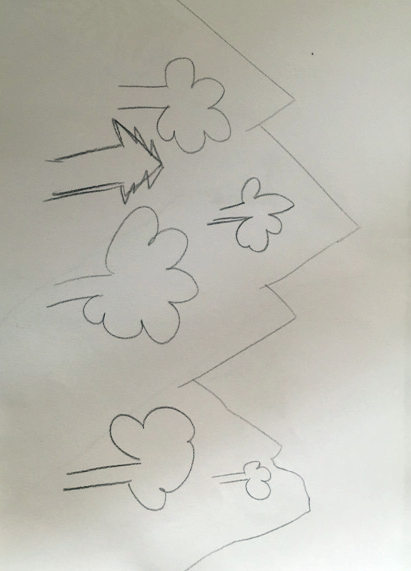
\includegraphics[angle=90, height=0.15\textheight]{images/croquis_2.jpg}&
    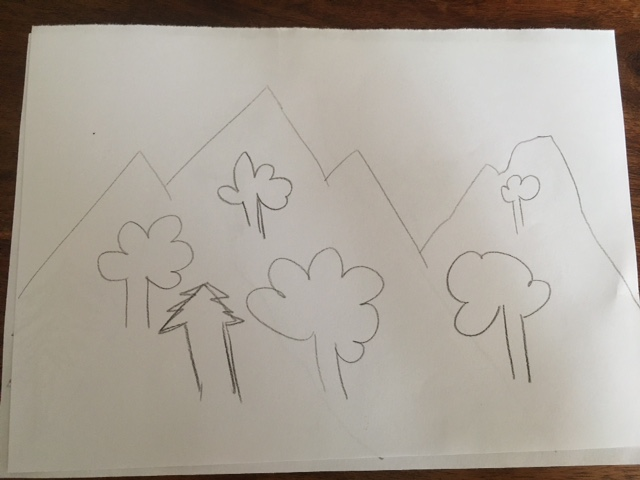
\includegraphics[angle=90, height=0.15\textheight]{images/croquis_4.jpg}\\
    (a)&(b)&(c)
  \end{tabular}
  \captionof{figure}{Dessin de paysages réalisés par des personnes différentes. On note que les niveaux d'informations sont plus ou moins élevés. Le dessin (b) est très abstrait tandis que nous observons plus de détails pour (a) .\label{fig-croquis}}
\end{center}



\chapter{Etat de l'art}
 
Nous présentons dans un premier temps les GANs qui sont au coeur de notre problématique. En un second lieu, nous étudions différents modèles existants basés sur les GANs conditionnels. Nous évoquons aussi, de manière plus succincte, des travaux liés à notre sujet mais n'utilisant pas les réseaux de neurones afin de pouvoir identifier les avantages et inconvénients des deux mondes. Nous terminons par une liste des datasets utiles à notre sujet.


\section{Généralités sur les GANs}

"Les GANs (en anglais generative adversarial networks) sont une classe d'algorithmes d'apprentissage non-supervisé. Ces algorithmes ont été introduits dès 2014 par Goodfellow et permettent de générer des images avec un fort degré de réalisme." \cite{wiki:Reseaux-antagonistes-generatifs}

Un générateur fabrique des données et les soumets au discriminateur dont le but est d'évaluer leurs degré de crédibilité. 

Le générateur $G(z, \theta_{1})$ représente un réseau de neurones capable de mapper du bruit $z$ vers l'espace désiré $x$. Le discriminateur $D(z, \theta_{2})$ retourne la probabilité dans l'intervalle $[0,1]$ que $x$ vient du dataset original. $\theta_{i}$ représente les poids définis par chacun des modèles. Le générateur tente de maximiser la probabilité que les données $x$, soient classifiées comme appartenant au dataset d'origine et inversement, le discriminateur minimise la probabilité que de fausses images appartiennent au dataset d'origine.

Il existe aujourd'hui une très grande variété de travaux de recherches basés les GANs (BCGAN, AmbientGAN, ORGAN, Perceptual GAN). Le dépôt "The GANs Zoo" \cite{hindupuravinash} référençait déjà en 2018 plus de 502 noms de GANs différents !


\section{CGANs et traduction d'image}

Les GANs conditionnels ajoutent une information supplémentaire $y$, partagée par le discriminateur et le générateur. Grâce aux cGANs il est possible de générer des images réalistes basées sur des labels de classes, des textes ou des images.

\subsection{Pix2Pix}
\cite{DBLP:journals/corr/GatysEB15a} nous montre en quoi les cGANs peuvent permettre de résoudre efficacement les problèmes de traductions d'images et propose un framework applicable à n'importe quel domaine.

\subsection{GauGan}
\cite{DBLP:journals/corr/abs-1903-07291} permet de générer des paysages réalistes basés sur des masques de segmentation sémantiques. Les auteurs introduisent la "normalisation conditionnel" ou "adaptative", permettant de prendre en compte notamment les informations spatials.
Les couches de normalisations ont tendances à faire perdre de l'information contenu dans les masques sémantiques d'entrées car ils ne dépendent pas de données externes.

\begin{center}
  \centering
  \begin{tabular}{cc}
    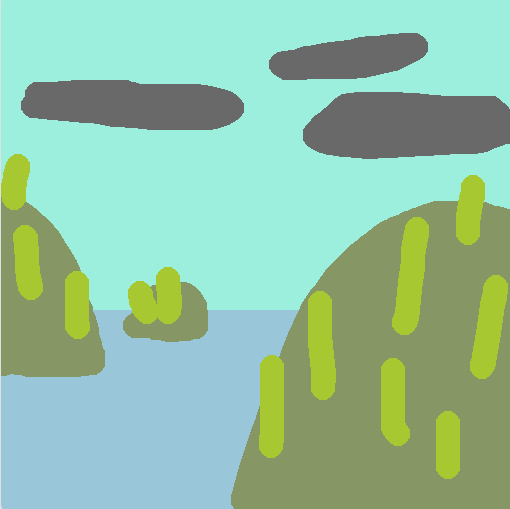
\includegraphics[height=0.15\textheight]{images/test-gaugan-sm.jpg}&
    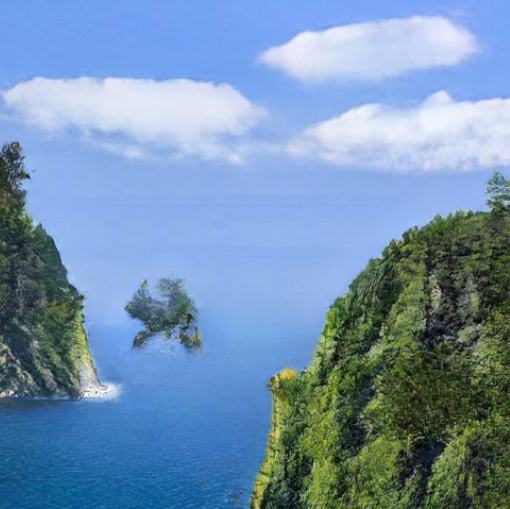
\includegraphics[height=0.15\textheight]{images/test-gaugan.jpg}\\
    (a) Input - masques de segmentation sémantiques &(b) Output
  \end{tabular}
  \captionof{figure}{Test de rendu de paysage à partir de l'application Gaugan : http://nvidia-research-mingyuliu.com/gaugan/\label{fig-gaugan}}
\end{center}



\subsection{Transfert de style neuronal} 
Introduit par Leon A. Gatys \cite{DBLP:journals/corr/GatysEB15a} le TDN consiste à transférer un style à partir d'une image de référence vers une image de contenu. L'objectif est de transformer l'image d'entrée (bruit) en minimisant la distance avec l'image de contenu et avec l'image de style. On obtient alors par rétropagation, une image qui correspond au contenu de l'image d'origine et au style souhaitée.

L'avantage de cette technique est quelle ne nécessite pas de dataset, seulement deux images sont nécessaires.

\begin{center}
  \centering
  \begin{tabular}{ccc}
    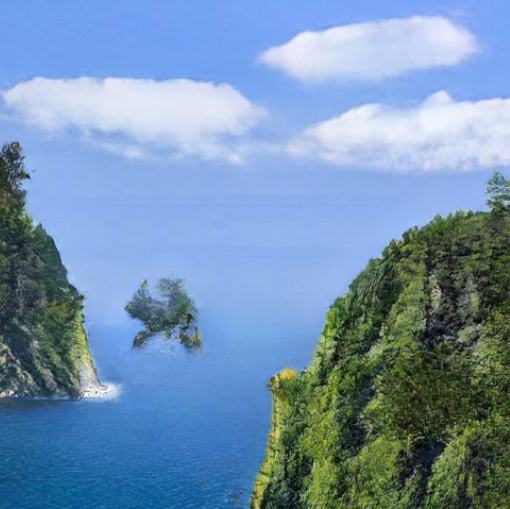
\includegraphics[height=0.15\textheight]{images/test-gaugan.jpg}&
    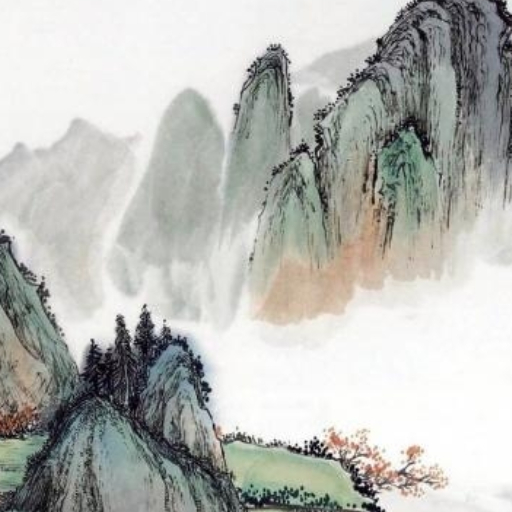
\includegraphics[height=0.15\textheight]{images/transfert-ds.jpg}&
    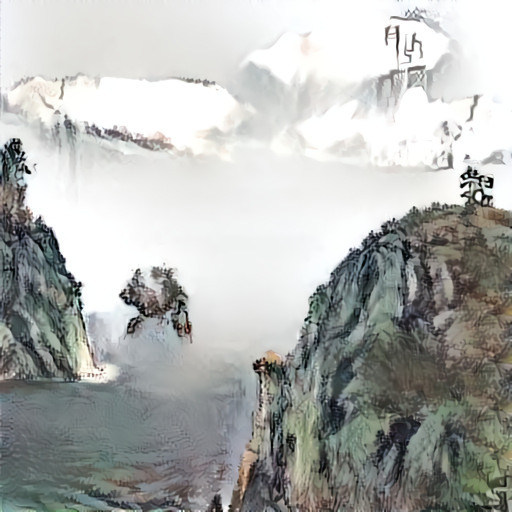
\includegraphics[height=0.15\textheight]{images/gaugan-tds.jpg}\\
    (a) Image de contenu & (b) Image de style &(c) Résultat
  \end{tabular}
  \captionof{figure}{Test de transfert de style réalisé à partir de la figure \ref{fig-gaugan}\label{fig-transfert-de-style}(b)}
\end{center}


\subsection{Learning to Sketch} 
\cite{DBLP:journals/corr/abs-1805-00247} présente une méthode permettant de transformer une photo en croquis, en essayant d'imiter la façon de faire d'un humain. Le modèle est capable de réaliser le croquis séquentiellement, c'est à dire trait par trait. Les auteurs proposent de résoudre le problème des styles subjectifs et variés des dessins humain en utilisant un modèle hybride supervisé/non-supervisé. L'objectif étant de palier "au signal de supervision faible et bruyant" induit par l'écart important entre un croquis et sa photo correspondante. \\

L'architecture est décomposé en 4 sous-modèles contenants chacun leur propres sous-réseaux d'encodeurs et de décodeurs. Deux réseaux supervisés traduisent respectivement une photo en croquis $D(E(photo))\to sketch$ et un croquis en photo $(D(E(sketch))\to photo)$ . Deux autres réseaux non-supervisés se chargent de la reconstruction. $D(E(photo))\to photo$ et $D(E(sketch))\to sketch$  \\


\subsection{Sketching: Inferring Contour Drawings from Images}
\cite{DBLP:journals/corr/abs-1901-00542} propose une nouvelle approche concernant la détection des contours dans une image. L'article montre que les solutions traditionnelles comme Canny \cite{4767851} , captent uniquement les signaux de haute fréquence dans l’image sans la comprendre. Les auteurs ont collecté un dataset de 5000 pairs "croquis humain/photos", crée manuellement via la plateforme de crowdsourcing "Amazon Mechanical Turk". En effet aucun dataset existant ne convenait (nombre d'éléments dans l'image, limites internes manquantes, le contenu non reconnaissable, les zones ombrées vides etc ..).

Ce modèle également du type "traduction image-image", permet d'avoir plusieurs labels différents pour la même photo, prenant en compte la nature subjective du dessin humain.

\section{Autre algorithmes n'utilisant pas le deep learning}
TODO


\section{Datasets disponibles}
Il est évident qu'il n'existe pas à l'heure actuel de dataset de paires abstraction/peinture chinoise.

\subsection{Croquis/abstractions}
Un des principal problème de la recherche dans le domaine de la génération de dessins à la main est le manque de dataset. Aujourd'hui les plus grosses bases de données que nous avons trouvées sont TU-Berlin \cite{eitz2012hdhso}, Sketchy \cite{sketchy2016} et Quickdraw. A noter que tous ces datasets sont constitués d'objets "isolés" et non composés comme peut l'être une peinture chinoise.

\subsection{Peinture chinoises}
"La peinture chinoise désigne toute forme de peinture originaire de Chine ou pratiquée en Chine ou par des artistes chinois hors de Chine." \cite{wiki:Peinture-chinoise} Il existe beaucoup de styles, courants et genres différentes (paysage, peinture narratives, faunes, flore, personnage). Nous prévoyons d'exploiter un dataset de plus de 5000 peintures chinoises au format 256x256, récupérées depuis \cite{ychen93}


\chapter{Propositions de solutions}

Malgré nos recherches, nous n'avons à ce jour trouvé aucun modèle nous permettant de réaliser totalement notre projet. Ci-dessous une liste non définitive des nouvelles pistes que nous souhaitons explorer.

\section{Création du dataset en semi automatique}

En utilisant le logiciel LabelBox, il est possible de labelliser manuellement une image à travers l'utilisation des sémantiques layout. A titre d'information, labelliser 1000 images prendrait environ 2 jours hommes à raison d'une minute par image. Une fois cette étape réalisée, nous pourrions générer une ou plusieurs abstractions pour chaque peintures, en utilisant le dataset "quick draw" entre autres. Outre l'inconvénient du temps passé, cette solution n'est pas généralisable.

\section{Photo-Sketching: Inferring Contour Drawings from Images}
Todo : Fakhri

\section{Abstraire une image via les RCNN}
Nous savons que les RCNNs, grâce aux couches de convolutions, sont capables de détecter les caractéristiques visuelles communes d'un ensemble d'images. Comme le prouve ce travail : https://medium.com/artists-and-machine-intelligence/perception-engines-8a46bc598d57, il est peut-être possible de générer un représentation abstraite de nos peintures en utilisant ce principe. Il serait alors théoriquement possible d'obtenir des pairs abstractions/peintures, permettant l'entraînement d'un cGAN type "traduction image-image". 

\chapter{Conclusion et Perspectives\label{chap-conclusion}}

\bibliographystyle{alpha}
\bibliography{memoire}
\end{document}
